
It is one thing to read a paper and understand something at a high level and it is another to actually implement the concept described. Here I will discuss my own efforts and struggles in implementing AlphaZero on smaller environments. I think it good to clear up some terminology confusion that can arise. When I say that I implemented AlphaZero and what most people mean when they talk about AlphaZero is the general concepts used to solve the game of Go. So this means that the specific hyperparameters or network architecture is not necessary implement your own version on a different environment. I will recap here what those core concepts of AlphaZero are. 

\begin{algorithm}[H]
\SetKwFunction{FSelfPlay}{SelfPlay}
\SetKwFunction{FTrainNetwork}{TrainNetwork}
\SetKwFunction{FEval}{Eval}
\SetAlgoLined
 init Network\;
 init ReplayBuffer;
 
 \For{iter in iters}{
  
  run \FSelfPlay
  
  run \FTrainNetwork
  
  run \FEval
  
 }
 \caption{AlphaZero Core}
  
\end{algorithm}

In Algorithm one above you can see that the algorithm can actually be condensed to a small number of parts. Each one of those parts has a lot going on but it helps to have a high level understanding of the algorithm before getting into the details. Let go through each piece. The first thing that happens is the network is randomly initialized. We refer to both policy and value networks as a single network. The algorithm is run for a predefined number of iterations. You could also have a stopping criterion if you wanted based on performance. For each iteration of the algorithm we do three main things. Self-play, network training and evaluation. The self play step is what generates the data for our network to train on. We play some predetermined number of games against ourselves. The results of those games are saved off for training the network. Playing against yourself here means that the role of player 1 and player 2 is assumed by the same AlphaZero agent and therefore the same network. Training the network means random sampling a batch of data from the replay buffer some number of epochs. The network is updated each epoch using backpropagation to minimize the loss function previously mentioned.  

\begin{equation}
    l = (v - z)^{2} - \pi^{T} \log{\hat{\pi_{\theta}}} + c||\theta||^{2}
\end{equation}

The final step is the evaluation step. In the AlphaGo Zero paper this was performed by keeping track of a best network. You keep a best network in memory and then after every time you update the current network you have your newly updated network play against the current best. If the current network beats the current best by a certain threshold then the current network is now set the best network otherwise the current network is discarded. So in this scheme you dont actually keep your updated network until it is able to beat the previous best version. In my own implementation I found that this hurt performance and I opted to continually update the network each iteration. This is actually what they do in their follow up paper AlphaZero \cite{alphagozero}. Lets look at self play in a little more detail. 


\begin{algorithm}[H]
\SetKwFunction{FSelfPlay}{SelfPlay}
\SetKwFunction{FMCTS}{MCTS}
\SetAlgoLined
\SetKwProg{Fn}{Def}{:}{}
 \Fn{\FSelfPlay{$Agent$,$NumberGames$}}{
    
    \For{game in Games}{
        
        reset Tree;
        
        reset Env; 
        
        \While{True}{
            
            $s_{t} \sim Env$ 
            
            $a \sim MCTS(s)$
            
            $s_{t}, a, s_{t + 1}, r, done \sim Env.next(s)$
            
            $Agent.StoreMemory(s_{t},a,r)$
            
            \If{done}{
                break;
            
            }
            
        \EndWhile
      }
    }
}
\end{algorithm}


A few things of note in the SelfPlay algorithm above. The first is that at the beginning of each game the tree is being reset. When the agent runs MCTS to select an action all of the statistics above the current node in the tree are forgotten about. It is possible to have different criterion for how often you reset the statisics in the tre but the idea is that old statistics were generated by an old network and therefore not as reliable. We will discuss specifics of MCTS and the different hyper parameters used later. We next give a brief look at the network training step. 

\begin{algorithm}[H]
\SetKwFunction{FTrainNetwork}{TrainNetwork}
\SetAlgoLined
\SetKwProg{Fn}{Def}{:}{}
 \Fn{\FTrainNetwork{$Agent$,$Epochs$}}{
    
    \For{epoch in Epochs}{
        $ s, \hat{\pi}, z \sim Agent.Memory$ \Command{Sample data from replay buffer that was created during self play}
        
        $ (\pi_{\theta} , v ) \sim Agent.NN(s) $ \Command{Pass s through the network}
        
        $ l = (z - v)^{2} + \pi^{T} \log{\hat{\pi_{\theta}}} + c||\theta||^{2}$
        
        $ \theta_{t} = \theta_{t -1} - \alpha \frac{\partial l}{\partial \theta}$
    }
}
\end{algorithm}


\subsection{TicTacToe Experiments}

Now that we have a reasonably good idea of what the high level logic looks I believe you should have a good idea of how the algorithm works. Lets look at a few experiments to try and get a better feel for how the algorithm works in practice. These first few set of experiments we will be running AlphaZero on the game of tictactoe. Tictactoe is played on a 3x3 grid. The players place pieces onto the grid with goal of connecting 3 in a row. You can connect 3 in row horizontally, vertically or diagonally. The game is nice because it is small enough that we can actually find optimal solutions. I will use the same neural network architecture for all of the experiments that follow. 

\textbf{NN Architecture}
\begin{itemize}
    \item Convolutional Layer with padding + BatchNorm
    \item Convolutional Layer with padding + BatchNorm
    \item Convolutional Layer + BatchNorm
    \item policy head is just a single fully connected layer with a log softmax as an activation function
    \item value head is also a fully connected layer but with $tanh$ as the activation function
\end{itemize}

You can see that there are no residual connections used here. This could certainly be added for improved performance but the goal here was to get use something small but still had some of the properties of what a larger application would need.  I did for instance use just a simple Neural architecture that only had fully connected layers and the performance seemed to suffer quite noticeably. If the reader is interested in attempting different architectures please go the github page linked to in the abstract. It is quite easy to change if desired. I used pytorch for building the network and for training the network. Pytorch \cite{pytorch} is an open source machine learning framework that is supposed to be used for "research to production". The VikingZero codebase does not depend heavily on the framework used and would not take much effort to swap out pytorch for tensorflow or something else. 

In the AlphaGo Zero paper the input to the network is an actual stack of frames. This is nice because it automatically encodes some temporal knowledge. In the VikingZero implementation I dont look back any time steps. So the input is a single frame for each player and then a layer representing whose turn it is. So here is what that looks like. 

\begin{figure}[H]
       \centering
       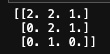
\includegraphics[width=100px,height=100px]{experiments/demo_board_1.png}
       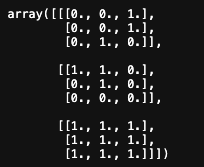
\includegraphics[width=100px,height=100px]{experiments/transform_demo_board.png}
       \caption{Left Figure is a tictactoe board. Figure on the right is the transformed version }
       \label{fig:my_label}
\end{figure}

Now lets discuss the relevant hyper parameters that require tuning. In the AlphaGo Zero paper they used Bayesian hyper parameter optimization to tune their network. I did not have that luxury and so I tuned the network "by hand". That basically just means you start with a best guess at an architecture, run an experiment, view the outcome, change a single hyperparameter and repeat. AlphaZero has a lot of hyperparameters which makes tuning it rather cumbersome. The list below is quite long but I hope that it helps demonstrate that it is not as simple as aiming the algorithm at a problem and hitting go and expecting good results. 

\textbf{Exploration parameters}
These are the hyper-parameters that changed how much exploration was done throughout training. First recall that actions during MCTS are selected by the following equation. 

\begin{equation}
    a_{t} = \underset{a}{argmax}(Q(s_{t},a) + U(s_{t},a))
\end{equation}

\begin{equation}
    U(s_{t},a) = c_{puct}P(s,a) \frac{\sqrt{\sum_{b}N(s,b)}}{1 + N(s,a)}
\end{equation}

More weight is given to $U(s,a)$ when N(s,a) is small relative to $\sum_{b}N(s,b)$. That is when the action $a$ associated with node $s$ has not been visited often relative to the other actions. More weight is given to $U(s,a)$ when the policy network $P(s,a)$ is larger. That means that the more opinionated the policy network becomes more likely it is to select that action during MCTS. This is a potential area for over fitting. 

\begin{itemize}
    \item \textbf{$c_{puct}$} This simply weights $U(s,a)$. Increasing $c_{puct}$ increases exploration. I found that the commonly used $\sqrt{2}$ was best. 
    \item \textbf{dirchlet noise}. This simply adds extra noise to the root of the search tree during MCTS and encourages additional exploration. This is \textbf{Not} used on any other nodes of tree other than the current root. Actions are then selected by
    $P(s,a) = (1 - \epsilon)p_{a} + \epsilon \eta_{a}$ where $\eta \sim Dir(\alpha_{d}$
    In my experiments I found that $epsilon = 0.1$ and $\alpha_{d}=0.03$ (same as paper) was best. Epsilon > 0.1 tended to cause too much variability in the action selected by MCTS resuliting in large variability during network training. 
    \item $\tau $ threshold. In the AlphaGo Zero paper actions against the actual environment are selected according to $\pi(a|s) = \frac{N(s,a)^{\frac{1}{\tau}}}{\sum_{b}N(s,b)^{\frac{1}{\tau}}}$ for a given number actions. After that given number of actions the action with the highest probability is selected. This translate into setting $\tau = 1$ during the beginning of play and then setting $tau -> 0$ once the agents has taken more actions than the threshold. I found that having the threshold = 3 in tictactoe worked well. 
\end{itemize}

\textbf{Network Parameters}

Now lets look at the hyperparameters w.r.t network training. 

\begin{itemize}
    \item \textbf{Optimizer}. Throughout these experiments I use the Adam optimizer provided by pytorch. In the paper they use SGD with momentum. I found that Adam outperformed for all of my experiments. 
    \item \textbf{lr} learning rate. The learning rate that I used was 0.001
    \item \textbf{Batch size}. This is how many samples are randomly sampled for each epoch of training. I used a batch size of 32 but found that sizes between [16,64] gave similar results. 
    \item \textbf{epochs}. See the \textbf{TrainNetwork} function above. Running 25 epochs worked best for me but this seemed like a bit large for a game like tictactoe but thats what worked best for me. 
    \item \textbf{Maxmemsize}. How much memory you allow to be kept in the replay buffer can have a significant affect on performance. For instance I kept a max size of 20k for a long time and then realized that this kept too much old data and did not allow the network to correctly capitalize on a newly "found" strategies. 
    
\end{itemize}

\textbf{More Parameters..}

\begin{itemize}
    \item \textbf{number of sims}. This refers to the number of times you run an iteration of MCTS from your root node. I found that running 25 simulations worked well. It was enough simulations that it gave your policy network a good target. Remember that running MCTS outputs $\hat{\pi}$ with the policy network tries to approximate. So if you dont run enough simulations $\hat{\pi}$ wont be very good. On the other hand running a lot is very costly computationally. So ideally you want the least number that is necessary to continuously be able to improve your policy network. 
    \item \textbf{number of games}. The number of games that you play (see Def SelfPlay) per iteration changes how much data that you end up generating. Generally in deep learning a lot of data is required. It is no different in this setting. If you dont play enough games than you wont have enough data to train on but if you play too many games you can end up overfitting to the current network. For tictactoe I found that playing 30 games was best. 
\end{itemize}

\textbf{Evaluation}

For evaluating the performance I used a few different metrics. The first metric was to play the agent vs a minimax agent and track the total score over iterations. For tictactoe this allowed me to get a comparison against an optimal agent. For Connect4 a minimax or full depth alphabeta agent was too slow. I used a depth limited alphabeta agent. Please see the Search section for a discussion on the alphabeta algorithm. The loss values for the policy and value networks are tracked every iteration. This is mostly to ensure the algorithm is actually learning. As we will see having a small error does not translate to winning. Another metric I used exclusively for the tictactoe experiments was an optimal play lookup. I used a minimax agent to look at every possible state and create a dictionary lookup of state --> action. The size of the dictionary is 4520. This ignores illegal positions and positions where the board is full since in that case there is no action to look at. To compare against the current agent I do an exhaustive comparison of the agents max actions vs the minimax action. I then report the mean score. This is an expensive test and so running it every iteration is not feasible but it gives a thorough look at the agents performance. 


\subsection{TicTacToe Experiments}

In these series of experiments we will show our best models performance and the hyperparameters used. We will then do a comparison vs other settings and do a side by side comparison. 

\textbf{Base model settings}

\begin{multicols}{2}

\begin{itemize}
    \item Batch size: 32
    \item $c_{puct}: 1.41$
    \item dirchlet noise: 0.03
    \item epochs: 25
    \item epsilon: 0.1

\end{itemize}

\begin{itemize}
    \item learning rate: 0.001
    \item max memory size: 5000
    \item number simulations: 25
    \item tau threshold: 3
    \item episodes: 300
    \item number training games: 30
\end{itemize}

\end{multicols}


\begin{figure}[H]
       \centering
       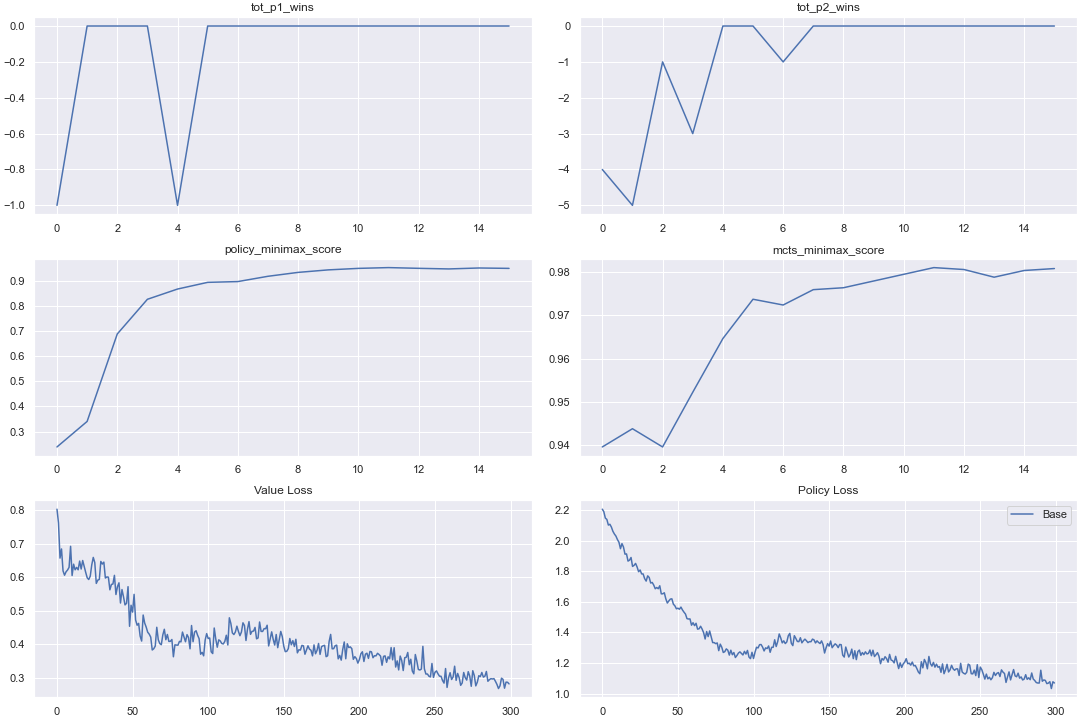
\includegraphics[width=400px,height=400px]{experiments/base_model.png}
       \caption{Base Case experiment}
       \label{fig:my_label}
\end{figure}

For the base case experiment looking at the figures left to right. tot\_p1\_wins is the total score out of 5 games. The agent gets a +1 for a win a -1 for a loss and 0 for a draw. Since minimax plays perfectly the best the agent can hope to do is get a score of 0. We can see that this is achieved fairly quickly from the perspective of player 1. From the perspective of player 2 we can see from the second figure that eventually the agent reaches a poit of always getting a draw vs minimax but is much more volitile at the beginning of training. The 




\textbf{Experiment 1}

In our first comparison we will look at the affect of the tau threshold on performance. Lowering the threshold equates to less variability in the data seen by the network. This in turn leads to less exploration in future iterations of training as the network learns to more quickly prefer those higher probability actions. This can lead to over fitting if there is not enough exploration in the MCTS portion of the algorithm. Below we show our base model in comparison with a model that has tau = 1 instead of 3. In this case there does seem to be over-fitting happening. We see from the loss graphs that the network quickly goes to having almost 0 loss. This would be good if we were doing supervised learning but here in the RL setting that does not always translate to a good outcome since we are generating our own dataset from interacting with the environment. The most striking difference I think here is looking at the "mcts\_minimax\_score". This shows how the tau=1 model quickly hits max performance and plateaus. We can also see that in performance vs minimax the tau=1 model was bouncing around quite a bit more. 

\begin{figure}[H]
       \centering
       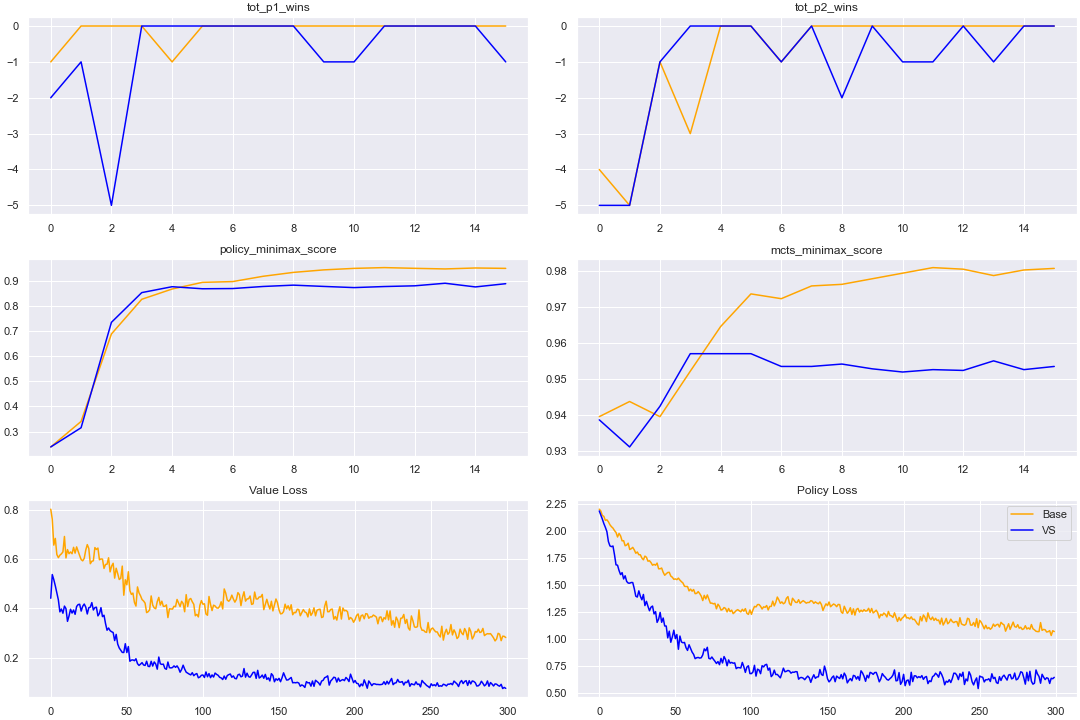
\includegraphics[width=400px,height=300px]{experiments/base_vs_t=2.png}
       \caption{Base vs tau = 1}
       \label{fig:my_label}
\end{figure}




\textbf{Experiment 2}

In this second comparison we will look at the affect of increasing the amount of noise during search by setting epsilon = 0.2. Recall that this increased noise happens only at the root of the search tree during MCTS. It seems that this model actually performs slightly better than our base model in the "mcts\_minimax\_score" but quite a bit more variability in its performance vs minimax. Not suprisingly the value and policy loss values are much higher. This is not surprising since we have a lot of variability in our training data. This highlights the point that increased exploration even if it comes at the cost of worse network performance might be worth it. 

\begin{figure}[H]
       \centering
       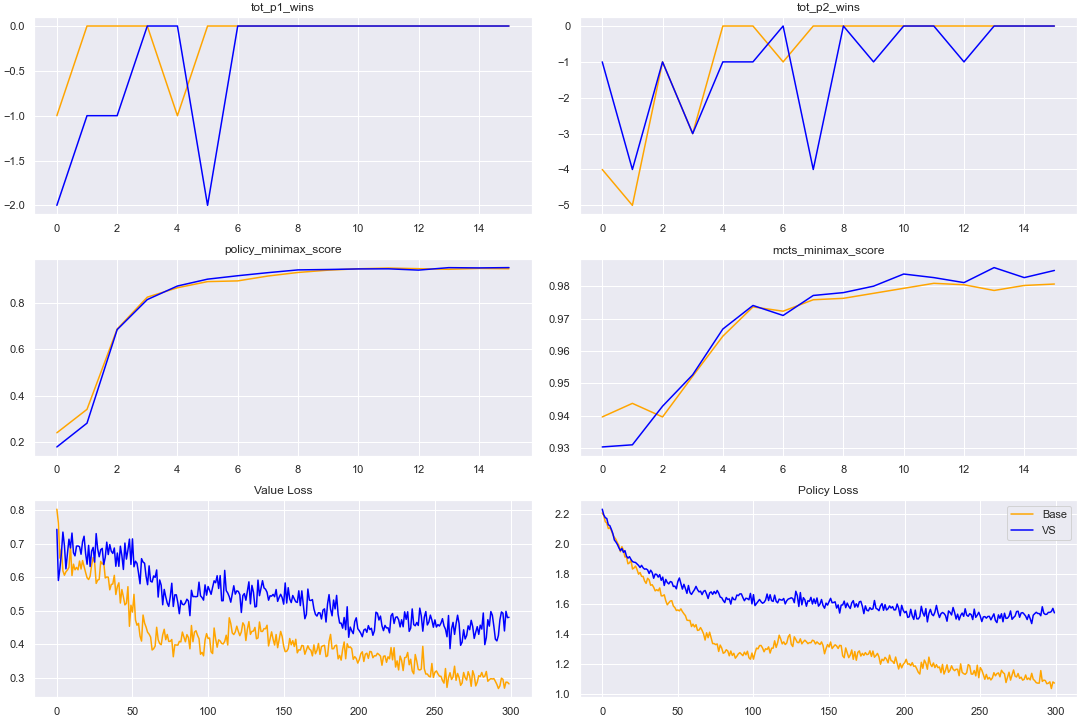
\includegraphics[width=400px,height=300px]{experiments/base_vs_eps=0_2.png}
       \caption{Base vs epsilon = 0.2}
       \label{fig:my_label}
\end{figure}



\textbf{Experiment 3}

In this third comparison we will look at the affect of decreasing the number of simulations performed during search. This really hurts performance more than any other metric. This was suprising to me given such a small environment such as tictactoe. It appears that even in non complex domains that a minimum amount of exploration is required and 15 simulations was not enough to both explore and exploit the better paths.  

\begin{figure}[H]
       \centering
       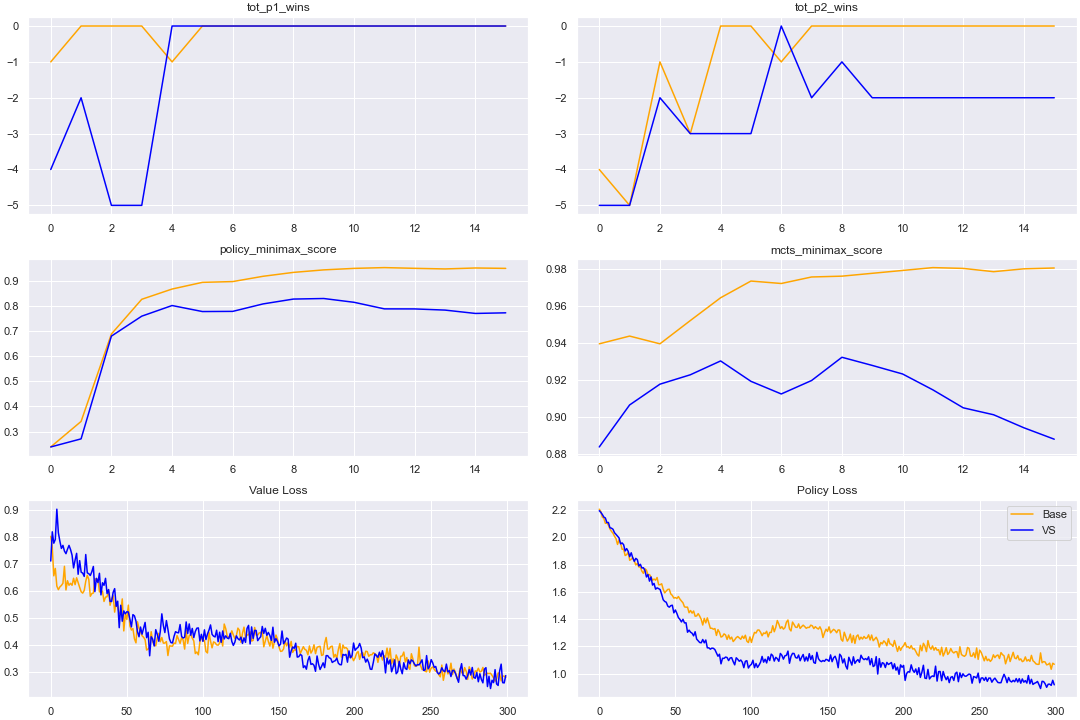
\includegraphics[width=400px,height=300px]{experiments/base_vs_nsim=15.png}
       \caption{Base vs nsim = 15}
       \label{fig:my_label}
\end{figure}


\textbf{Experiment 4}

In this fourth comparison we will look at the affect of increasing the number of games played per episode as well as increasing the maximum memory size. Here we set the max memory to 20000 and we play 50 games per iteration. This of course generates much more data than previous and allows us to keep more in memory. This should help to prevent over-fitting. Playing more games equates to seeing more board positions especially when the network is less certian about withc is best. Here we found that we did not increase performance and might have even hurt performance slightly. From the experiments that we ran it seemed however that this is something that will require a good amount of tuning. Large domains of course will require much more training data and will require you to hold on to older data for longer as well. 

\begin{figure}[H]
       \centering
       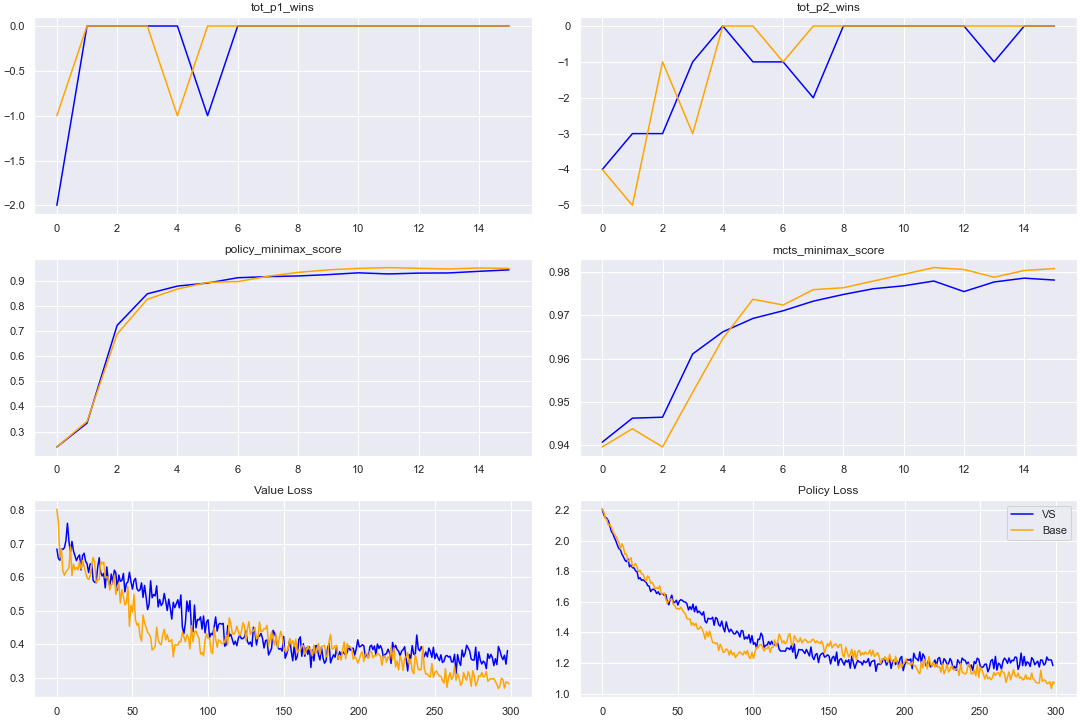
\includegraphics[width=400px,height=300px]{experiments/base_vs_maxmem.png}
       \caption{Base Case vs maxmem size}
       \label{fig:my_label}
\end{figure}


\textbf{Experiment 5}

Lets now look at an interesting experiment in which we increase the number of epochs the network runs. In the base case we run 25 and so what should doubling them do? My first guess was that it was going to over-fit and I am sure there is some high number of epoochs that you could run that would cause that to happen but I found that doubling the number of epochs actually seemed to help performance. The player 1 performance vs minimax immediately goes to optimal and stays there for the rest of training. The policy and mcts minimax scores are both better as well. 

\begin{figure}[H]
       \centering
       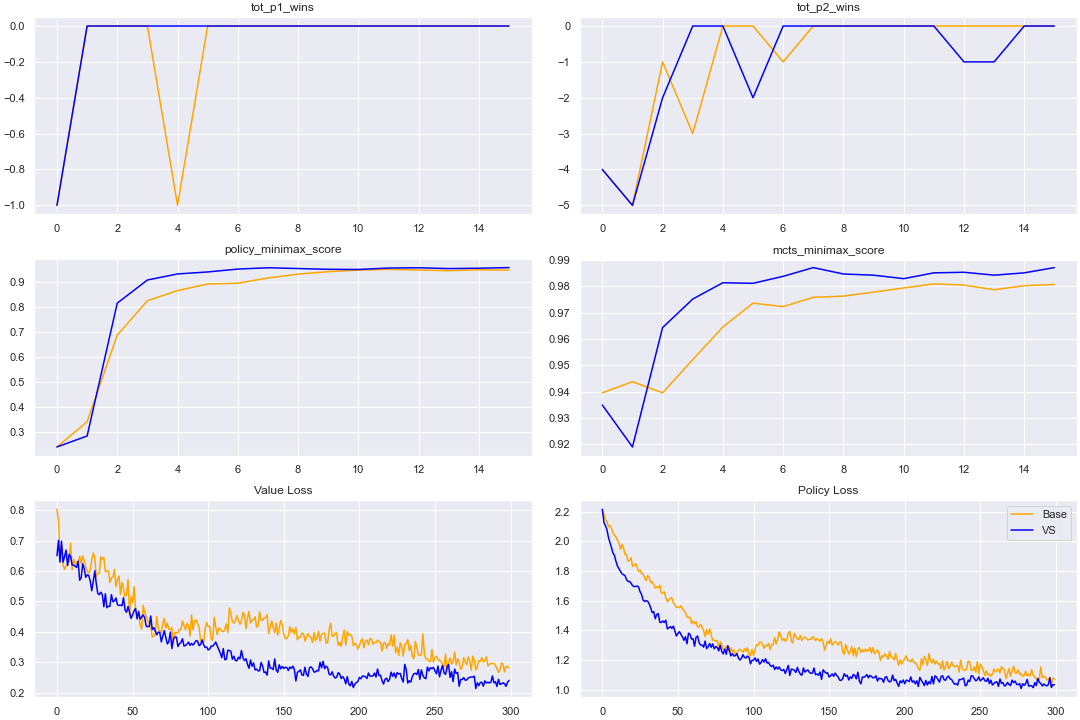
\includegraphics[width=400px,height=300px]{experiments/base_vs_epochs=50.png}
       \caption{Base Case vs Epochs =50}
       \label{fig:my_label}
\end{figure}


\subsection{Connect4 Experiments}

Lets now look at how our implementation does on the game of connect4. In these tests we were not able to use the minimax scores that we could do with tictactoe since we needed a dictionary action lookup over the full state space. So we will drop those tests. The game of connect 4 is the same as tictactoe expect the goal is to get 4 in a row instead of 3. It is played on a 6 x 7 board. 

\textbf{Parameters}

\begin{multicols}{2}

\begin{itemize}
    \item Batch size: 64
    \item max memory size: 20000
    \item number simulations: 35

\end{itemize}

\begin{itemize}
    \item tau threshold: 10
    \item number training games: 20
\end{itemize}

\end{multicols}

\begin{figure}[H]
       \centering
       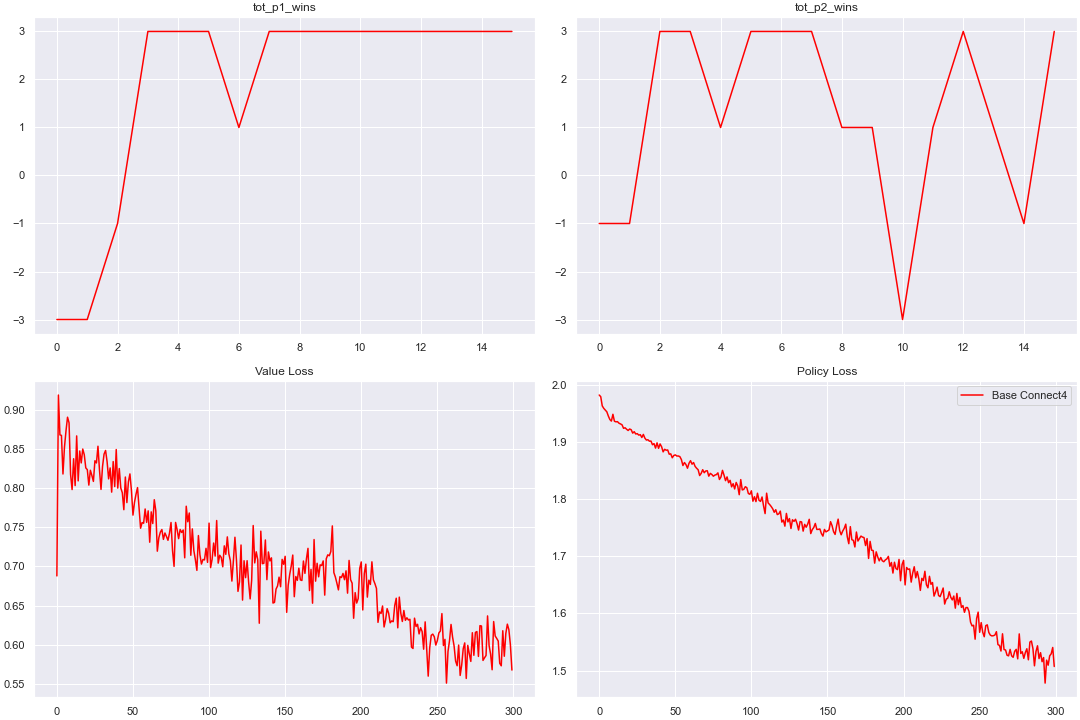
\includegraphics[width=400px,height=300px]{experiments/base_connect4.png}
       \caption{Base Case vs Epochs =50}
       \label{fig:my_label}
\end{figure}